%%%%%%%%%%%%%%%%%%%%%%%%%%%%%%%%%%%%%%%%%%%%%%%%%%%%%%%%%%%%%%%%%%%%%%%%%%%%%%%%
% DUET ICRA 2026 draft.
% Based on the official Papercept ieeeconf template downloaded from:
% https://ras.papercept.net/conferences/support/files/ieeeconf.zip
%%%%%%%%%%%%%%%%%%%%%%%%%%%%%%%%%%%%%%%%%%%%%%%%%%%%%%%%%%%%%%%%%%%%%%%%%%%%%%%%

\documentclass[letterpaper, 10 pt, conference]{ieeeconf}

\IEEEoverridecommandlockouts
\overrideIEEEmargins

\usepackage{amsmath}
\usepackage{amssymb}
\usepackage{booktabs}
\usepackage{graphicx}
\usepackage{multirow}
\usepackage[table]{xcolor}
\usepackage{url}
\usepackage{balance}
\usepackage{placeins}

\title{\LARGE \bf
DUET: Endogenous Failure Detection and Recovery via Dual-Action Disagreement
}

\author{Anonymous Authors% <-this % stops a space
% \thanks{This paper is an ICRA 2026 draft. Author names and affiliations are omitted for anonymous review.}
}

\begin{document}

\maketitle
\thispagestyle{empty}
\pagestyle{empty}

\begin{abstract}
Vision-language-action (VLA) policies fine-tuned on limited successful demonstrations can struggle to detect and recover from out-of-distribution (OOD) execution deviations. Existing solutions often add an external detector or require costly recovery data. We introduce DUET, a dual-action-head framework trained without failure or recovery trajectories. A state-conditioned relative head provides nominal control, while an absolute head without explicit proprioceptive conditioning predicts RVQ-conditioned return waypoints. After converting each waypoint into a local correction, its disagreement with the relative command, together with a state-bound violation score, continuously gates the two predictions. On four LIBERO suites and four failure families, DUET improves nominal success from $93.8\%$ to $96.9\%$ and action-perturbation success from $27.9\%$ to $64.6\%$ over its relative-only baseline. Disagreement also attains the best AUROC ($0.845$) among the evaluated success-only detectors. On a separately trained $\pi_0$ controller and Franka arm, DUET preserves $90.0\%$ nominal success and raises robot-state OOD success from $10.0\%$ to $77.5\%$.
\end{abstract}

\begin{figure*}[t]
\centering
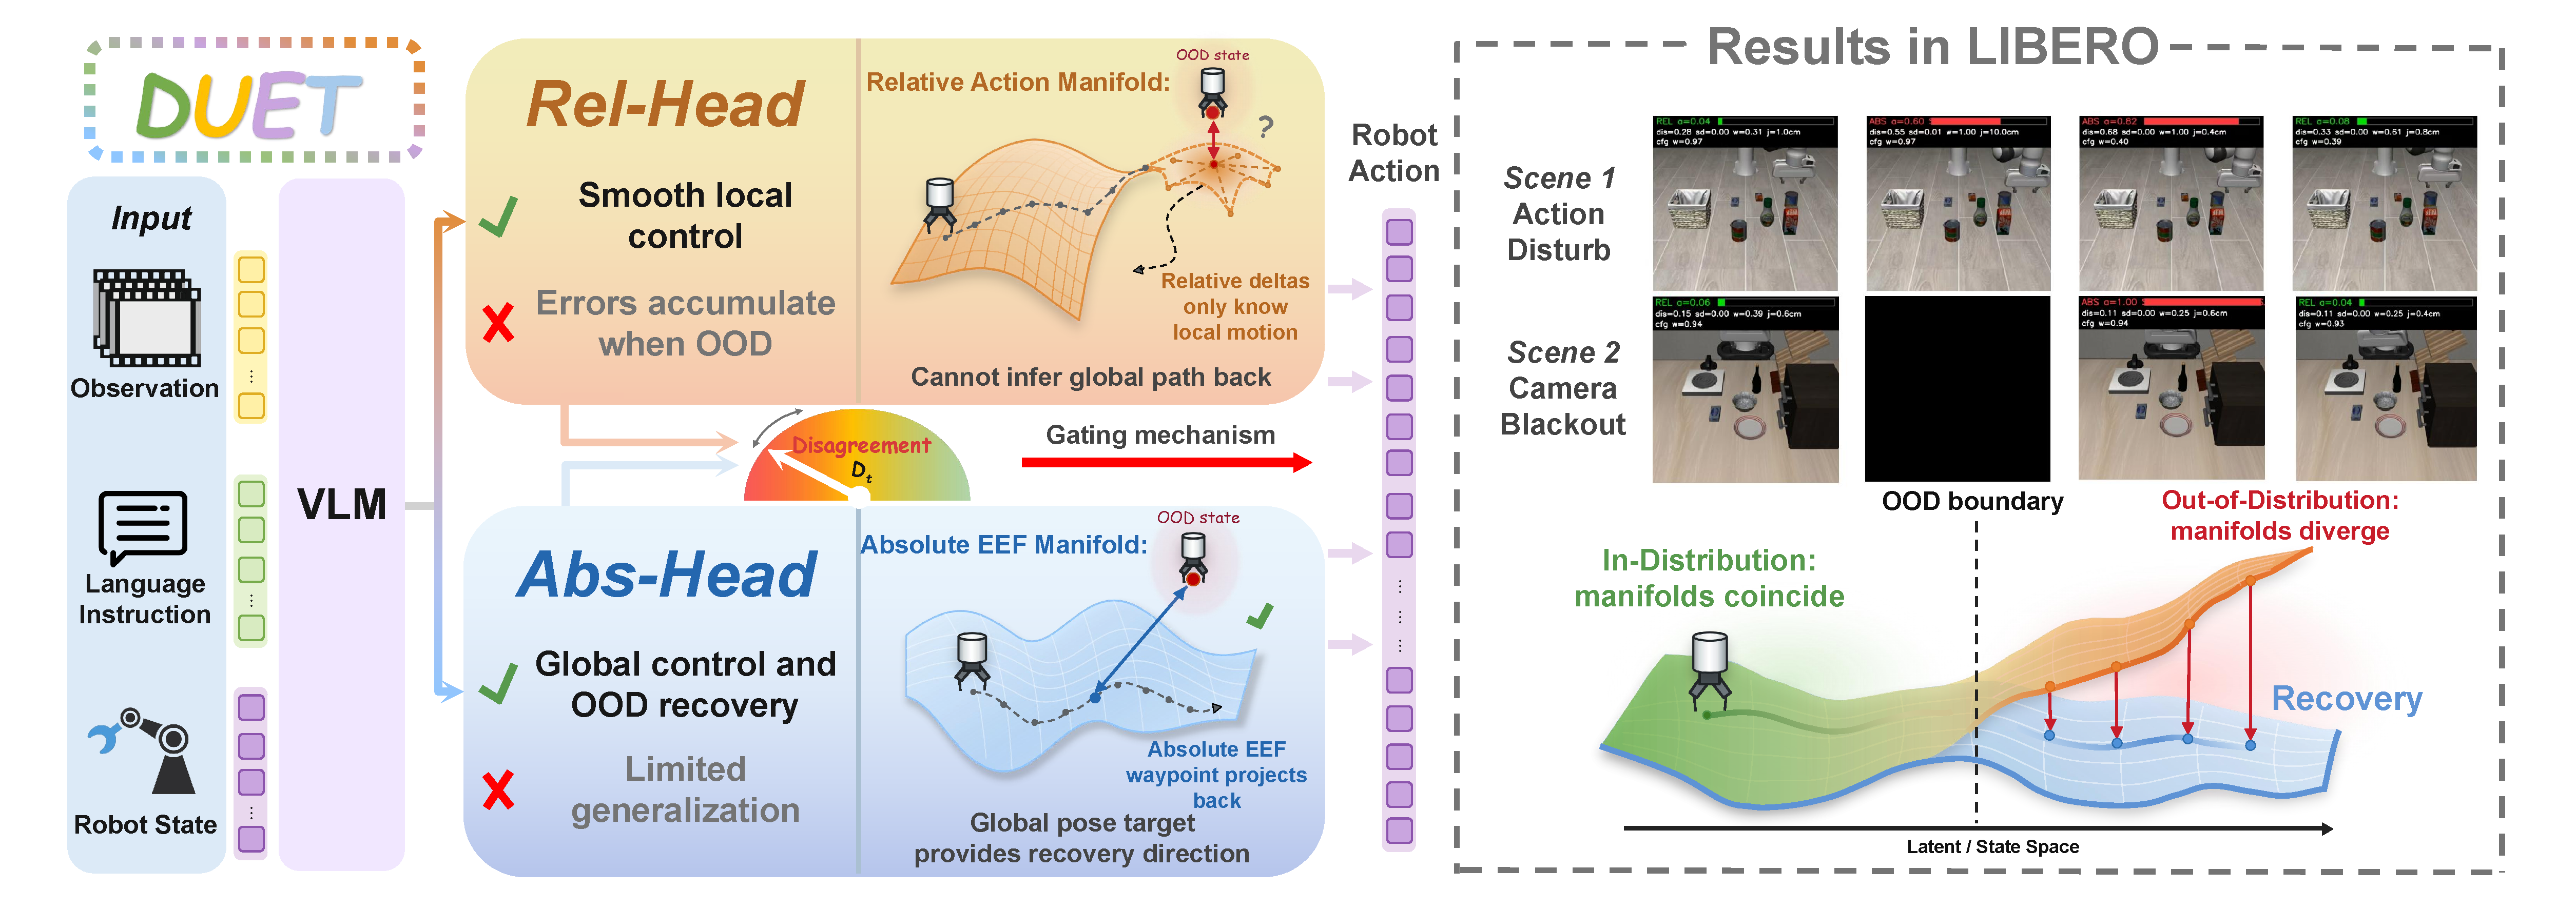
\includegraphics[width=0.96\textwidth]{figures/fig1.pdf}
\caption{DUET overview. Cross-space disagreement scores execution deviations and gates relative control with absolute-waypoint correction.}
\label{fig:teaser}
\end{figure*}

\section{INTRODUCTION}

Vision-language-action (VLA) policies adapt pretrained vision-language models to map visual observations and language instructions to robot actions \cite{openvla,starvla}. Trained on successful demonstrations, they can drift during closed-loop execution until task completion becomes unreliable---an \emph{execution failure}. Before failure becomes irreversible, the rollout may leave the observations, configurations, or action consequences supported by demonstrations. We call this an \emph{execution deviation}. An unexpected arm displacement changes the starting pose, while a dropped object changes the robot--object configuration even if the instruction remains unchanged. Deviation and failure are not equivalent: unseen states may still be handled successfully, while compounding errors can cause failure under familiar observations. We focus on deviations that elevate failure risk but remain recoverable by returning toward demonstrated behavior.

To anticipate failures and recover from these execution deviations, existing methods often train an external failure predictor \cite{faildetect} and a separate recovery controller using human takeovers or expert interventions \cite{dagger,sirius,intervengen}. Their supervision remains loosely coupled: the detector raises an alarm, while the controller depends on costly corrective data. We ask whether a VLA can use its own action predictions to detect a recoverable deviation and generate a retry direction from successful demonstrations alone, without an external failure model or recovery data.

Achieving this poses two coupled challenges. Successful demonstrations teach a policy how to act along successful trajectories, but do not explicitly teach it when its actions become unreliable or how to return after leaving those trajectories. Detection must therefore derive a meaningful risk signal from the policy itself, while recovery must infer a corrective direction from demonstrations that do not cover the encountered deviation. Our approach is motivated by a recurring observation from prior experiments: with large-scale training data, relative actions often yield the best performance by enabling stronger generalization. However, after fine-tuning on a small demonstration set, relative-action policies struggle to recover autonomously once execution enters out-of-distribution states. Absolute actions exhibit the complementary tradeoff: they generalize less effectively in the large-data regime but more readily guide execution back toward demonstrated behavior after a deviation under limited-data fine-tuning. This observation motivates DUET, which combines a relative head for nominal execution with an absolute head for trajectory re-entry. Disagreement between the relative command and the correction toward the absolute waypoint signals rising failure risk, while the waypoint itself supplies a retry direction.

The two heads learn matched future actions from each successful demonstration. The relative head receives the live robot state, whereas the absolute head excludes explicit proprioception to retain a scene-conditioned reference. Converting its waypoint into a correction from the measured pose makes the predictions comparable: they can agree along demonstrated trajectories yet separate after displacement, indicating both a mismatch and a candidate return direction.

The module attaches to shared vision-language features and is trained on StarVLA \cite{starvla} in simulation and $\pi_0$ (OpenPi) \cite{pi0} on hardware. At inference, a soft gate shifts toward waypoint correction as disagreement rises and restores relative control after realignment. Irreversible failures, hardware faults, and cases requiring a new task strategy remain outside its scope.

Our contributions are threefold:
\begin{itemize}
    \item We formulate failure-aware retry using cross-space disagreement as an endogenous failure-risk signal. The action heads require no failure labels, and the resulting score outperforms the evaluated success-only detectors on TPR and AUROC (\S\ref{sec:detection}).
    \item We propose DUET, unifying endogenous failure-risk scoring and waypoint-based correction while preserving smooth nominal control (\S\ref{sec:nominal}, \S\ref{sec:retry}).
    \item We evaluate DUET on StarVLA in LIBERO and on a separately trained $\pi_0$ (OpenPi) controller across four Franka tasks to test its applicability across backbones (\S\ref{sec:retry}, \S\ref{sec:real_robot}).
\end{itemize}

% Keep the abstract and introduction together on the opening page.
\section{RELATED WORK}

\subsection{Runtime Failure Detection}
Runtime monitors use model uncertainty, action inconsistency, or semantic progress. Sentinel combines temporal consistency with VLM-based progress assessment; we evaluate its training-free STAC signal \cite{sentinel}. FAIL-Detect performs sequential OOD detection without failure examples using policy likelihoods or success-only features; we compare its logpZO, RND, and PCA-kmeans variants \cite{faildetect}. These scalar alarms indicate when to intervene, but not how. DUET instead compares a relative command with the local correction induced by a success-trained waypoint, so the paired predictions provide both a risk score and a recovery direction.

\subsection{Recovery from Execution Failures}
One route expands the training distribution. DAgger queries experts on policy-induced states \cite{dagger}; intervention learning obtains corrective actions from human takeovers \cite{eil,sirius}; and IntervenGen synthesizes trajectories from a small intervention set \cite{intervengen}. RACER combines recovery demonstrations, language, and VLM supervision \cite{racer}, while optimized VLM prompts support motion or task-level correction \cite{vlmrecovery}. These methods can address failures requiring new semantic decisions, but add supervision, intervention, or inference machinery.

Recovery can also reuse existing demonstrations. Back to the Manifold returns toward high-density training states \cite{backtomanifold}, and OCR learns an inverse recovery policy from object-keypoint structure \cite{ocr}. Rewind-IL returns to VLM-verified demonstration checkpoints \cite{rewindil}; FAR performs test-time adaptation using failure-derived preferences \cite{far}. Avoiding recovery demonstrations is therefore not unique to DUET. Its distinction is that two action representations learned jointly from successful trajectories supply both the trigger and a closed-loop waypoint correction, without an external detector, checkpoint retrieval, or test-time update.

\subsection{Action Representations for Robust Control}
Action-space design affects policy learning, transfer, and closed-loop stability \cite{aljalbout2024actionspace,feng2026demystifying}. Prior comparisons largely select one representation for nominal prediction. DUET retains two views: state-conditioned relative commands for local execution and image-conditioned absolute waypoints as return targets. Their asymmetric conditioning is operational: disagreement signals inconsistency between local execution and the visually inferred target, while the waypoint remains usable for correction.

\section{METHOD}

\subsection{Problem Formulation}
At time $t$, the robot observes multi-view images $o_t$, a language instruction $l$, and proprioceptive state $s_t$. Trained only on successful demonstrations, DUET predicts the same behavior in two action representations over a horizon $K$:
\begin{align}
    \hat{\Delta A}_t &= f_{\mathrm{rel}}(o_t,l,s_t)
    \in \mathbb{R}^{K\times 7}, \\
    \hat{W}_t &= f_{\mathrm{abs}}(o_t,l)
    \in \mathbb{R}^{K\times 7}.
\end{align}
$\Delta A_t$ contains relative operational-space commands and $W_t$ absolute waypoints $[x,y,z,r_x,r_y,r_z,g]$. Recorded deltas and future end-effector states supervise the respective heads. Fusion acts on the 6-D pose component $a_p$; the deployed gripper command comes from the relative head.

Paired labels describe the same demonstrated continuation, so neither head requires annotated failures or recovery actions. Below, $\hat{\delta a}_{p,t}$ and $\hat{w}_{p,t}$ denote the current elements of the predicted chunks. The live pose converts the absolute target into a correction but is not an explicit input to the absolute predictor.

\begin{figure}[!t]
\centering
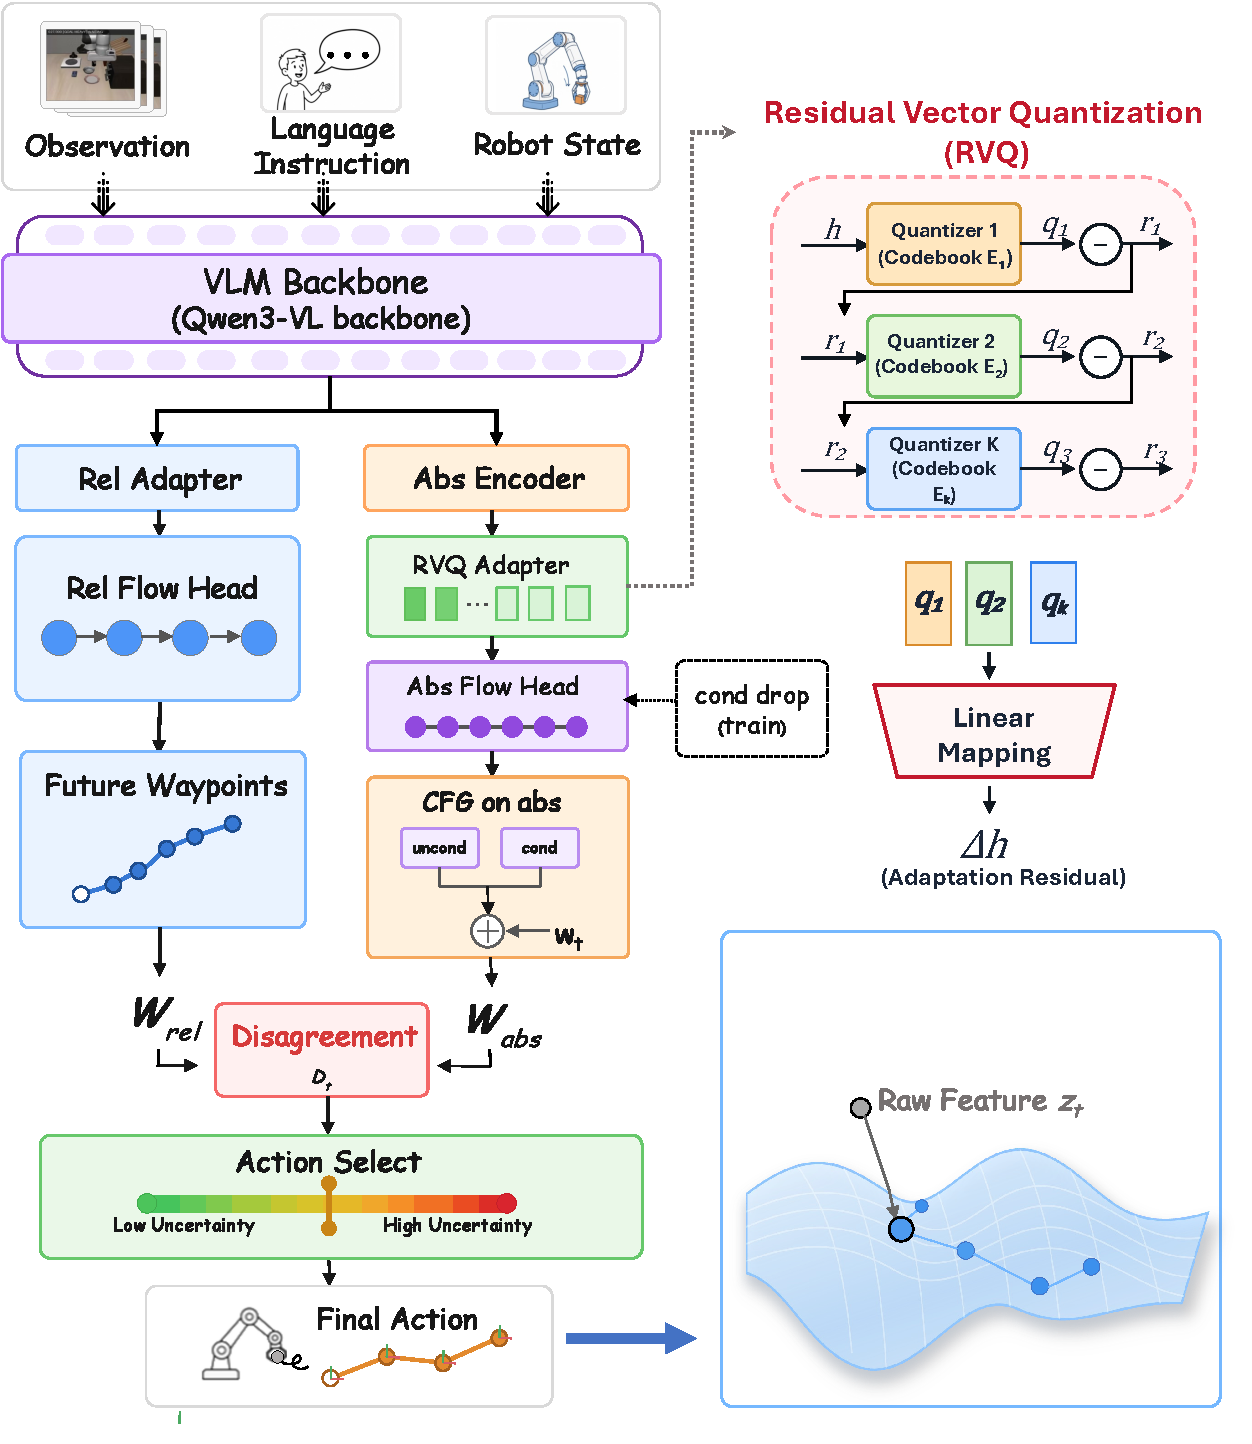
\includegraphics[width=\columnwidth]{figures/fig2.pdf}
\caption{DUET architecture: shared encoder, relative and RVQ-anchored absolute heads, and disagreement-gated recovery.}
\label{fig:architecture}
\end{figure}

\subsection{Dual-Action Views of Successful Behavior}
\label{sec:dual_views}
For instruction $l$, let $\mathcal{S}_l$ denote the region of robot execution represented by successful demonstrations. This support is only an interpretation of the training distribution: DUET neither estimates a geometric manifold nor optimizes a manifold-alignment objective. The relative head answers \emph{how to move next} from live pose $p_t$,
\begin{equation}
    \hat{\delta a}_{p,t} = f_{\mathrm{rel}}(o_t,l,s_t)_p,
\end{equation}
which is locally precise but provides no return destination off support. The absolute head answers \emph{where to be},
\begin{equation}
    \hat{w}_{p,t}=f_{\mathrm{abs}}(o_t,l)_p,
\end{equation}
providing a coarser target anchored by successful demonstrations.

We map the waypoint to a one-step correction at the live pose,
\begin{equation}
    c_t=\Psi_{p_t}(\hat{w}_{p,t}),
    \label{eq:command_conversion}
\end{equation}
instantiated in Eq.~\eqref{eq:recovery_vector} by normalized translation and geodesic rotation residuals. This is a command-space conversion, not parallel transport or an explicit geometric alignment on $SE(3)$.

Raw deltas and absolute coordinates cannot be compared directly: a robot displacement changes the correction required to reach a waypoint even when that waypoint remains unchanged. Expressing both predictions in local command units separates this execution mismatch from their different output parameterizations.

On support, $c_t$ and $\hat{\delta a}_{p,t}$ describe the same behavior and should broadly agree. Off support, local extrapolation can diverge from the demonstrated anchor. We use their residual as a heuristic---not calibrated---failure score and $c_t$ as its implied recovery direction. Disagreement is neither necessary nor sufficient for failure: corrupted observations can degrade both heads together, as handled in Sec.~\ref{sec:method-gate}. We therefore validate it empirically in Sec.~\ref{sec:detection}.

\subsection{Dual-Head Architecture}
Figure~\ref{fig:architecture} shows the shared VLM and two flow-matching heads \cite{diffusionpolicy,pi0}. The relative head attends to the full sequence and receives $s_t$. The absolute head excludes state tokens from pooling, preserving a complementary observation-conditioned reference rather than a second state-conditioned local controller.

It pools the hidden sequence $H^0$ after excluding explicit state tokens and applies residual vector quantization (RVQ) \cite{vqvae,rvq}:
\begin{equation}
    Z_q=\operatorname{RVQ}\!\left(\operatorname{Pool}(H^0)\right).
\end{equation}
The quantized representation is a discrete conditioning bottleneck learned from successful demonstrations. Its residual norm is auxiliary telemetry. Classifier-free guidance (CFG) \cite{cfg} modulates the contribution of conditional information during recovery.

The bottleneck is not a lookup of recorded recovery trajectories. Quantized features condition the absolute head, which still predicts the waypoint; quantization does not guarantee that an off-support target is reachable or task-correct.

\subsection{Disagreement-Preserving Learning}
\label{sec:learning}
Both heads train on paired labels from every successful trajectory, with flow-matching objectives and an RVQ commitment loss:
\begin{equation}
    \mathcal{L} =
    \lambda_{\mathrm{rel}}\mathcal{L}_{\mathrm{rel}}
    + \lambda_{\mathrm{abs}}\mathcal{L}_{\mathrm{abs}}
    + \lambda_{\mathrm{vq}}\mathcal{L}_{\mathrm{vq}},
\label{eq:training_loss}
\end{equation}
where absolute labels are normalized future states and relative labels are recorded deltas. We omit cross-head consistency loss to preserve useful disagreement.

Agreement on successful behavior is encouraged indirectly by paired supervision. Explicitly forcing agreement on perturbed inputs could suppress the very residual used for monitoring; the separate objectives instead allow the branches to respond differently when their conditioning becomes unreliable.

Asymmetric visual augmentation specializes the branches. With probability $p_{\mathrm{aug}}$, each view receives one or two of color jitter, an $80$--$95\%$ resized crop, and Gaussian pixel noise ($\sigma{=}5$--$25$ on $[0,255]$); targets remain unchanged. The relative head is optimized only on the clean subset $\mathcal{B}_{\mathrm{clean}}$:
\begin{equation}
    \mathcal{L}_{\mathrm{rel}} =
    \frac{1}{|\mathcal{B}_{\mathrm{clean}}|}
    \sum_{i \in \mathcal{B}_{\mathrm{clean}}}
    \ell_{\mathrm{FM}}(\hat{\Delta A}^{(i)}, \Delta A^{(i)}).
\end{equation}
The absolute and RVQ losses use the full batch, while the relative loss excludes augmented samples. This keeps the relative head sensitive and the absolute branch robust. For CFG, the absolute head replaces its quantized condition by learned null tokens on a subset of samples.

\subsection{Joint Failure-Risk Scoring and Recovery}
\label{sec:method-gate}
At deployment the policy returns both unnormalized action chunks. With live pose $p_t=(x_t,R_t)$ and absolute waypoint $\hat{w}_{p,t}=(\hat{x}_t,\hat{R}_t)$, the command conversion in Eq.~\eqref{eq:command_conversion} is
\begin{equation}
    c_t=\operatorname{clip}\!\left(
    \begin{bmatrix}
    (\hat{x}_t-x_t)/\sigma_p \\
    \operatorname{Log}^{\vee}(\hat{R}_tR_t^{-1})/\sigma_R
    \end{bmatrix},-1,1\right),
    \label{eq:recovery_vector}
\end{equation}
where $\operatorname{Log}^{\vee}:SO(3)\rightarrow\mathbb{R}^3$ returns the rotation vector used by the controller. We use $\sigma_p{=}0.05$\,m and $\sigma_R{=}0.5$\,rad, matching the operational-space controller scales that map a unit command to translation and rotation. Cross-space disagreement is the primary failure-risk signal,
\begin{equation}
    D_t=\frac{\left\|c_t-
    \operatorname{clip}(\hat{\delta a}_{p,t},-1,1)\right\|_2}{\sqrt{6}}.
    \label{eq:disagreement}
\end{equation}
The factor $\sqrt{6}$ makes $D_t$ a root-mean-square command discrepancy across pose dimensions. Since both compared vectors are clipped componentwise, $D_t\in[0,2]$; it is a discrepancy scale, not a failure probability. Translation and rotation are compared only after conversion by their respective action scales.
A coarse state-distance term measures normalized violation of the training-state bounds. Let $u_t\in\mathbb{R}^7$ be the measured absolute end-effector state in the same coordinates as the waypoint labels (translation, canonicalized rotation vector, and gripper position), let $u_{\min},u_{\max}$ be its coordinatewise training bounds, and let $[z]_+=\max(z,0)$. Then
\begin{equation}
    S_t =
    \frac{1}{7}\sum_{j=1}^{7}\left[
    \frac{[u_{\min,j}-u_{t,j}]_+ + [u_{t,j}-u_{\max,j}]_+}
    {\max(u_{\max,j}-u_{\min,j},\epsilon)}
    \right].
\end{equation}
We use $\epsilon{=}10^{-6}$. The failure-risk score and recovery weight are $q_t = D_t + \lambda S_t$ and $\alpha_t = \sigma(k(q_t-\tau))$. DUET interpolates local execution and global recovery while keeping relative gripper control:
\begin{align}
    a_t &= [a_{p,t},a_{g,t}], \\
    a_{p,t} &= (1-\alpha_t)\hat{\delta a}_{p,t} + \alpha_t c_t, \\
    a_{g,t} &= \hat{\delta a}_{g,t},
    \label{eq:fused_action}
\end{align}
Relative control dominates on support; rising $q_t$ shifts the pose command toward $c_t$, and control returns after realignment. The previous fusion weight from a valid observation sets the next absolute-head CFG scale, $w_t = w_{\max}-(w_{\max}-w_{\min})\alpha_{t-1}$. Thus $q_t$ determines \emph{when} and $c_t$ \emph{how} to recover. If vision is invalid, a guard freezes the last reliable waypoint and holds $\alpha_t{=}1$ until it returns; this guard override is not fed back into CFG.

\section{EXPERIMENTS}
\label{sec:experiments}

\begin{samepage}
We organize the simulation experiments around three questions:
\begin{itemize}
    \setlength{\itemsep}{0pt}
    \setlength{\parsep}{0pt}
    \setlength{\topsep}{2pt}
    \item[\textbf{(Q1)}] \textbf{Failure-aware retry:} Can DUET recover from controlled execution deviations and complete the task?
    \item[\textbf{(Q2)}] \textbf{Baseline comparison:} Does DUET improve robustness without sacrificing nominal performance?
    \item[\textbf{(Q3)}] \textbf{Endogenous failure-risk scoring:} Does cross-space disagreement provide a useful runtime signal for recoverable execution failures when the action heads are trained only on successful demonstrations?
\end{itemize}
Closed-loop success is the primary outcome. We evaluate disturbed execution, nominal performance, and detection quality, then use ablations and hardware experiments to test the mechanism and its applicability across backbones.
\end{samepage}

\subsection{Evaluation Protocol}
\label{sec:protocol}
We evaluate four LIBERO suites \cite{libero}, each with $10$ tasks and $50$ initial states per task, using checkpoints trained only on successful demonstrations ($10$k steps for Spatial, Object, and Goal; $40$k for LIBERO-10). Training uses seed $42$, AdamW, $500$ warmup steps, and cosine decay; the base/interface/head learning rates are $2.5{\times}10^{-5}/10^{-5}/10^{-4}$, and both flow heads use four inference steps.

StarVLA \cite{starvla} is the external relative-action baseline. DUET-Rel ($\alpha_t{=}0$) and DUET share a checkpoint, so their difference isolates adaptive recovery, whereas StarVLA$\to$DUET-Rel captures dual-head co-training. Absolute-only ($\alpha_t{=}1$) and fixed fusion ($\alpha_t{=}0.5$) are inference-time ablations. DUET uses Qwen3-VL features (size $2048$), 16-/8-layer relative/absolute DiT-B heads, and $K{=}8$ actions per chunk. The absolute branch uses $16$ RVQ tokens from three codebooks (size $512$, dimension $256$), with $p_{\mathrm{aug}}{=}0.3$, $p_{\mathrm{drop}}{=}0.15$, $\lambda{=}1$, $\tau{=}0.5$, $k{=}8$, and $(w_{\min},w_{\max}){=}(0,1)$. These gate settings are fixed across suites and perturbations.

Perturbations use deterministic seeds and matched $(\mathrm{task},\mathrm{initial\ state})$ keys. At step $5$, action perturbation replaces the six pose-command dimensions by a seeded random unit vector scaled to $0.5/0.8$ for $10/15$ steps at medium/severe intensity, while preserving the gripper command. At step $39$, EEF teleport applies a collision-checked random XY displacement of $5/8$\,cm while preserving height and orientation. A medium grasp drop lowers the held object by $5$\,cm at step $67$. At step $23$, blackout replaces both third-person and wrist images by zeros for $15/30$ steps. These fixed steps place disturbances in initial reach, transport, post-grasp, and approach, respectively. They ensure identical interventions across methods but sample one recovery horizon per family. All perturbed episodes remain in the success-rate denominator; we report injection coverage for semantic preconditions and use paired McNemar tests.

\begin{table}[t]
\caption{Failure families and affected OOD quantities.}
\label{tab:taxonomy}
\centering
\resizebox{\columnwidth}{!}{%
\begin{tabular}{lll}
\toprule
Family & Protocol & What becomes OOD \\
\midrule
Action execution & Action perturbation (step $5$) & Command-to-motion map \\
Robot displacement & EEF teleport (step $39$) & Robot-arm pose \\
Object / grasp & Vertical grasp drop (step $67$) & Robot--object configuration \\
Visual occlusion & Camera blackout (step $23$) & Current visual observation \\
\bottomrule
\end{tabular}}
\end{table}

\begin{figure}[t]
\centering
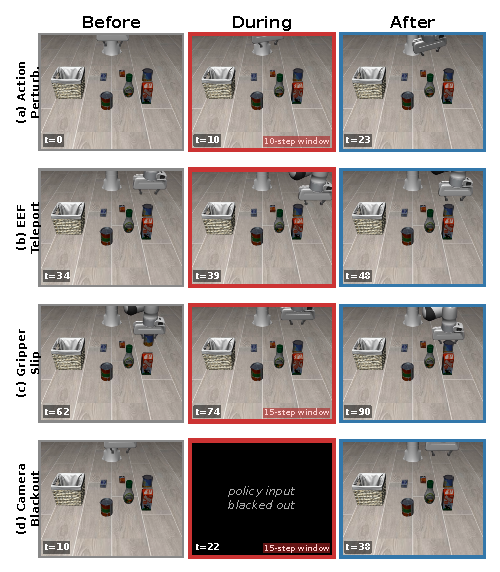
\includegraphics[width=\columnwidth]{figures/fig_perturbation_showcase.pdf}
\caption{Object-suite disturbances, before/during/after: (a) action perturbation, (b) EEF teleport, (c) grasp drop, (d) camera blackout.}
\label{fig:showcase}
\end{figure}

\begin{table*}[!t]
\caption{Post-intervention task success (\%; $N{=}500$/cell). Overall rows pool medium and severe conditions across all suites.}
\label{tab:ood_detailed}
\centering
\footnotesize
\begin{tabular*}{\textwidth}{@{\extracolsep{\fill}} l cccc @{\hspace{1.2em}} cccc @{}}
\toprule
& \multicolumn{4}{c}{Medium} & \multicolumn{4}{c}{Severe} \\
\cmidrule(lr){2-5}\cmidrule(l){6-9}
Suite & StarVLA & Rel. & DUET & $\Delta$ & StarVLA & Rel. & DUET & $\Delta$ \\
\midrule
\multicolumn{9}{@{}l}{\textit{(i) Action perturbation (step $5$)}} \\
Spatial    & 60.0 & 54.0 & 74.0 & $+20.0$ & 14.0 & 12.8 & 43.2 & $+30.4$ \\
Object     & 41.6 & 48.8 & 84.4 & $+35.6$ &  7.8 &  7.8 & 60.6 & $+52.8$ \\
Goal       & 52.2 & 47.2 & 74.2 & $+27.0$ & 18.8 & 10.6 & 52.6 & $+42.0$ \\
LIBERO-10  & 36.2 & 36.6 & 78.6 & $+42.0$ &  6.2 &  5.4 & 49.0 & $+43.6$ \\
\textbf{Overall} & 29.6 & \textbf{27.9} & \textbf{64.6} & $\mathbf{+36.7}$ & \multicolumn{4}{c}{\textit{med$+$sev combined}} \\
\midrule
\multicolumn{9}{@{}l}{\textit{(ii) EEF teleport (step $39$)}} \\
Spatial    & 55.4 & 54.6 & 57.6 & $+3.0$  & 46.8 & 48.2 & 52.6 & $+4.4$ \\
Object     & 43.4 & 36.2 & 76.0 & $+39.8$ & 21.2 & 20.8 & 68.4 & $+47.6$ \\
Goal       & 41.6 & 33.4 & 52.4 & $+19.0$ & 30.4 & 28.2 & 50.6 & $+22.4$ \\
LIBERO-10  & 40.4 & 35.8 & 60.8 & $+25.0$ & 21.4 & 18.4 & 56.8 & $+38.4$ \\
\textbf{Overall} & 37.6 & \textbf{34.5} & \textbf{59.4} & $\mathbf{+24.9}$ & \multicolumn{4}{c}{\textit{med$+$sev combined}} \\
\midrule
\multicolumn{9}{@{}l}{\textit{(iii) Vertical grasp drop (Object only, medium, step $67$)}} \\
Object     & 90.6 & 89.2 & \textbf{95.2} & $\mathbf{+6.0}$  & \multicolumn{4}{c}{---} \\
\midrule
\multicolumn{9}{@{}l}{\textit{(iv) Camera blackout (step $23$)}} \\
Spatial    & 81.0 & 88.0 & 94.4 & $+6.4$  & 42.4 & 63.2 & 95.2 & $+32.0$ \\
Object     & 91.8 & 96.8 & 98.6 & $+1.8$  & 64.2 & 95.0 & 97.2 & $+2.2$ \\
Goal       & 65.4 & 86.0 & 86.4 & $+0.4$  & 35.4 & 65.8 & 85.8 & $+20.0$ \\
LIBERO-10  & 60.0 & 65.6 & 84.2 & $+18.6$ & 24.4 & 25.6 & 86.2 & $+60.6$ \\
\textbf{Overall} & 58.1 & \textbf{73.5} & \textbf{90.8} & $\mathbf{+17.3}$ & \multicolumn{4}{c}{\textit{med$+$sev combined}} \\
\bottomrule
\end{tabular*}
\end{table*}

\subsection{\textbf{(Q1)} Failure-Aware Retry}
\label{sec:retry}
Table~\ref{tab:ood_detailed} reports rollout success, not success conditioned on detection. Against shared-checkpoint DUET-Rel, DUET improves action perturbation from $27.9\%$ to $64.6\%$, displacement from $34.5\%$ to $59.4\%$, grasp loss from $89.2\%$ to $95.2\%$, and occlusion from $73.5\%$ to $90.8\%$, exceeding StarVLA in every aggregate. Disabling fusion at inference isolates online correction from co-training.

\emph{Action and robot displacement.} DUET gains $36.7$ pp under action perturbation and $24.9$ pp under teleport. The scene remains observable, consistent with the absolute branch supplying a return target when relative commands become unreliable. Gains persist at both severities but vary by suite: severe Object teleport improves by $47.6$ pp, whereas Spatial gains only $3.0/4.4$ pp ($p{=}0.21/0.067$, not significant). The remaining recovery horizon limits interpretation of the latter result.

\emph{Grasp and vision.} A $5$\,cm drop yields a significant $6.0$ pp gain from an $89.2\%$ baseline ($p{=}2.4{\times}10^{-5}$; coverage $\geq98.8\%$). Restoring arm pose need not restore a changed grasp. During blackout, the validity guard freezes the last reliable waypoint; its aggregate gain is therefore evidence for the full robustness system rather than disagreement-based failure detection alone.

\begin{figure}[t]
\centering
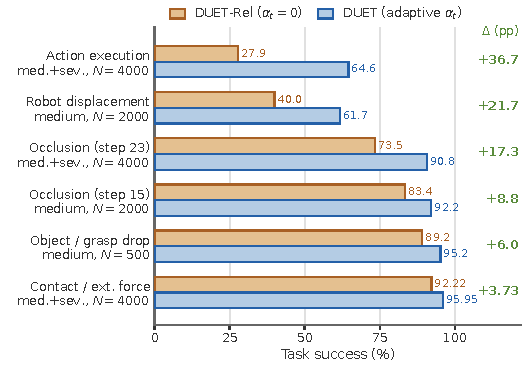
\includegraphics[width=\columnwidth]{figures/fig_ood_overall_success.pdf}
\caption{Paired DUET-Rel$\to$DUET gains by failure family.}
\label{fig:overall}
\end{figure}

\paragraph{Mechanism evidence}
Figure~\ref{fig:telemetry} shows transient recovery: arm-state disturbances raise disagreement and correction weight; after realignment, relative control resumes. World-state responses are weaker, while complete visual dropout invokes the guard. These traces support the switching mechanism, but do not imply that every disagreement peak predicts failure.

\begin{figure}[t]
\centering
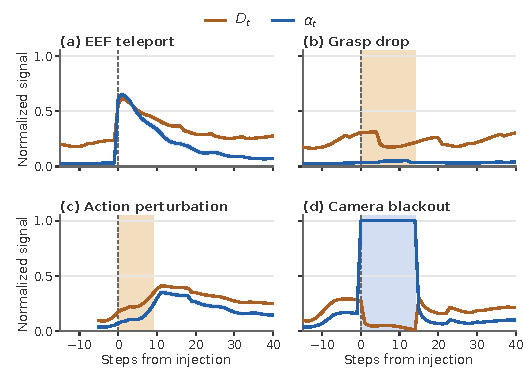
\includegraphics[width=\columnwidth]{figures/fig_ood_mechanism_grid.pdf}
\caption{Injection-aligned $D_t,\alpha_t$ on Object (mean, pointwise 95\% CI): (a,c) arm-state OOD, (b) world-state change, (d) validity guard.}
\label{fig:telemetry}
\end{figure}

For the geometric analysis in Fig.~\ref{fig:manifold}, the task-conditioned reference set $\mathcal{R}_{\ell}\subset\mathbb{R}^3$ contains end-effector positions from successful, unperturbed Object rollouts collected before scoring the disturbed rollouts. We measure translational distance to this set as $d_{\mathcal{M}}(t)=\min_{x^{\mathrm{ref}}\in\mathcal{R}_{\ell}}\lVert x_t-x^{\mathrm{ref}}\rVert_2$; orientation and gripper state are excluded. Re-entry occurs at the first post-injection step for which $d_{\mathcal{M}}(t)\leq3$\,cm, and re-entry time is measured from the injection at step $39$. On the trace-complete subsets ($n{=}484$--$498$), DUET closes $4.69$\,cm within $32$ steps and re-enters in $97.9\%$ of episodes (median $16$ steps), versus $0.71$\,cm, $62.5\%$, and $58$ steps for DUET-Rel. Absolute-only reaches $99.6\%$ re-entry but only $1.1\%$ task success. These subset rates differ slightly from the all-rollout rates in Table~\ref{tab:ood_detailed}. Geometric proximity is insufficient without resuming task-appropriate local actions.

\begin{figure}[t]
\centering
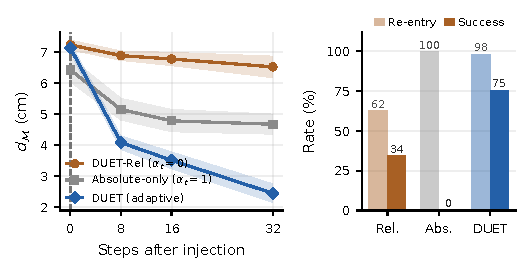
\includegraphics[width=\columnwidth]{figures/fig_manifold_distance.pdf}
\caption{Object teleport (medium, step $39$; trace-complete $n{=}484$--$498$). Left: clean-trajectory distance. Right: subset re-entry and task success.}
\label{fig:manifold}
\end{figure}

Together these results answer \textbf{Q1}: DUET converts recoverable deviations into successful retries, while grasp changes and invalid vision bound disagreement alone.

\subsection{\textbf{(Q2)} Baseline Comparison}
\label{sec:nominal}
Table~\ref{tab:nominal} shows that adaptive fusion raises nominal success from $93.8\%$ to $96.9\%$ at fixed capacity and training data, improving every suite. Larger gains on Goal ($92.0\%\to97.6\%$) and LIBERO-10 ($86.0\%\to91.8\%$) suggest correction of naturally accumulating errors, although success rates do not identify their cause. DUET matches the reported $\pi_{0.5}$ average and exceeds the StarVLA-GR00T average by $0.4$ pp. Differences in backbone and training protocol make both external rows contextual rather than controlled comparisons.

\begin{table}[t]
\caption{Nominal LIBERO success (\%). $\pi_{0.5}$: reported OpenPI $30$k checkpoint; StarVLA-GR00T: joint $30$k training; DUET: suite-specific $10$k/$40$k checkpoints.}
\label{tab:nominal}
\centering
\resizebox{\columnwidth}{!}{%
\begin{tabular}{lccccc}
\toprule
Method & Spatial & Object & Goal & LIBERO-10 & Avg. \\
\midrule
$\pi_{0.5}$ (reported) \cite{pi05} & 98.8 & 98.2 & 98.0 & 92.4 & 96.9 \\
StarVLA-GR00T \cite{starvla} & 97.8 & 98.8 & 97.4 & 92.0 & 96.5 \\
\midrule
DUET-Rel ($\alpha_t{=}0$) & 98.0 & 99.2 & 92.0 & 86.0 & 93.8 \\
\rowcolor{gray!20}
DUET & 98.8 & 99.4 & 97.6 & 91.8 & \textbf{96.9} \\
\bottomrule
\end{tabular}}
\end{table}

\begin{figure*}[!t]
\centering
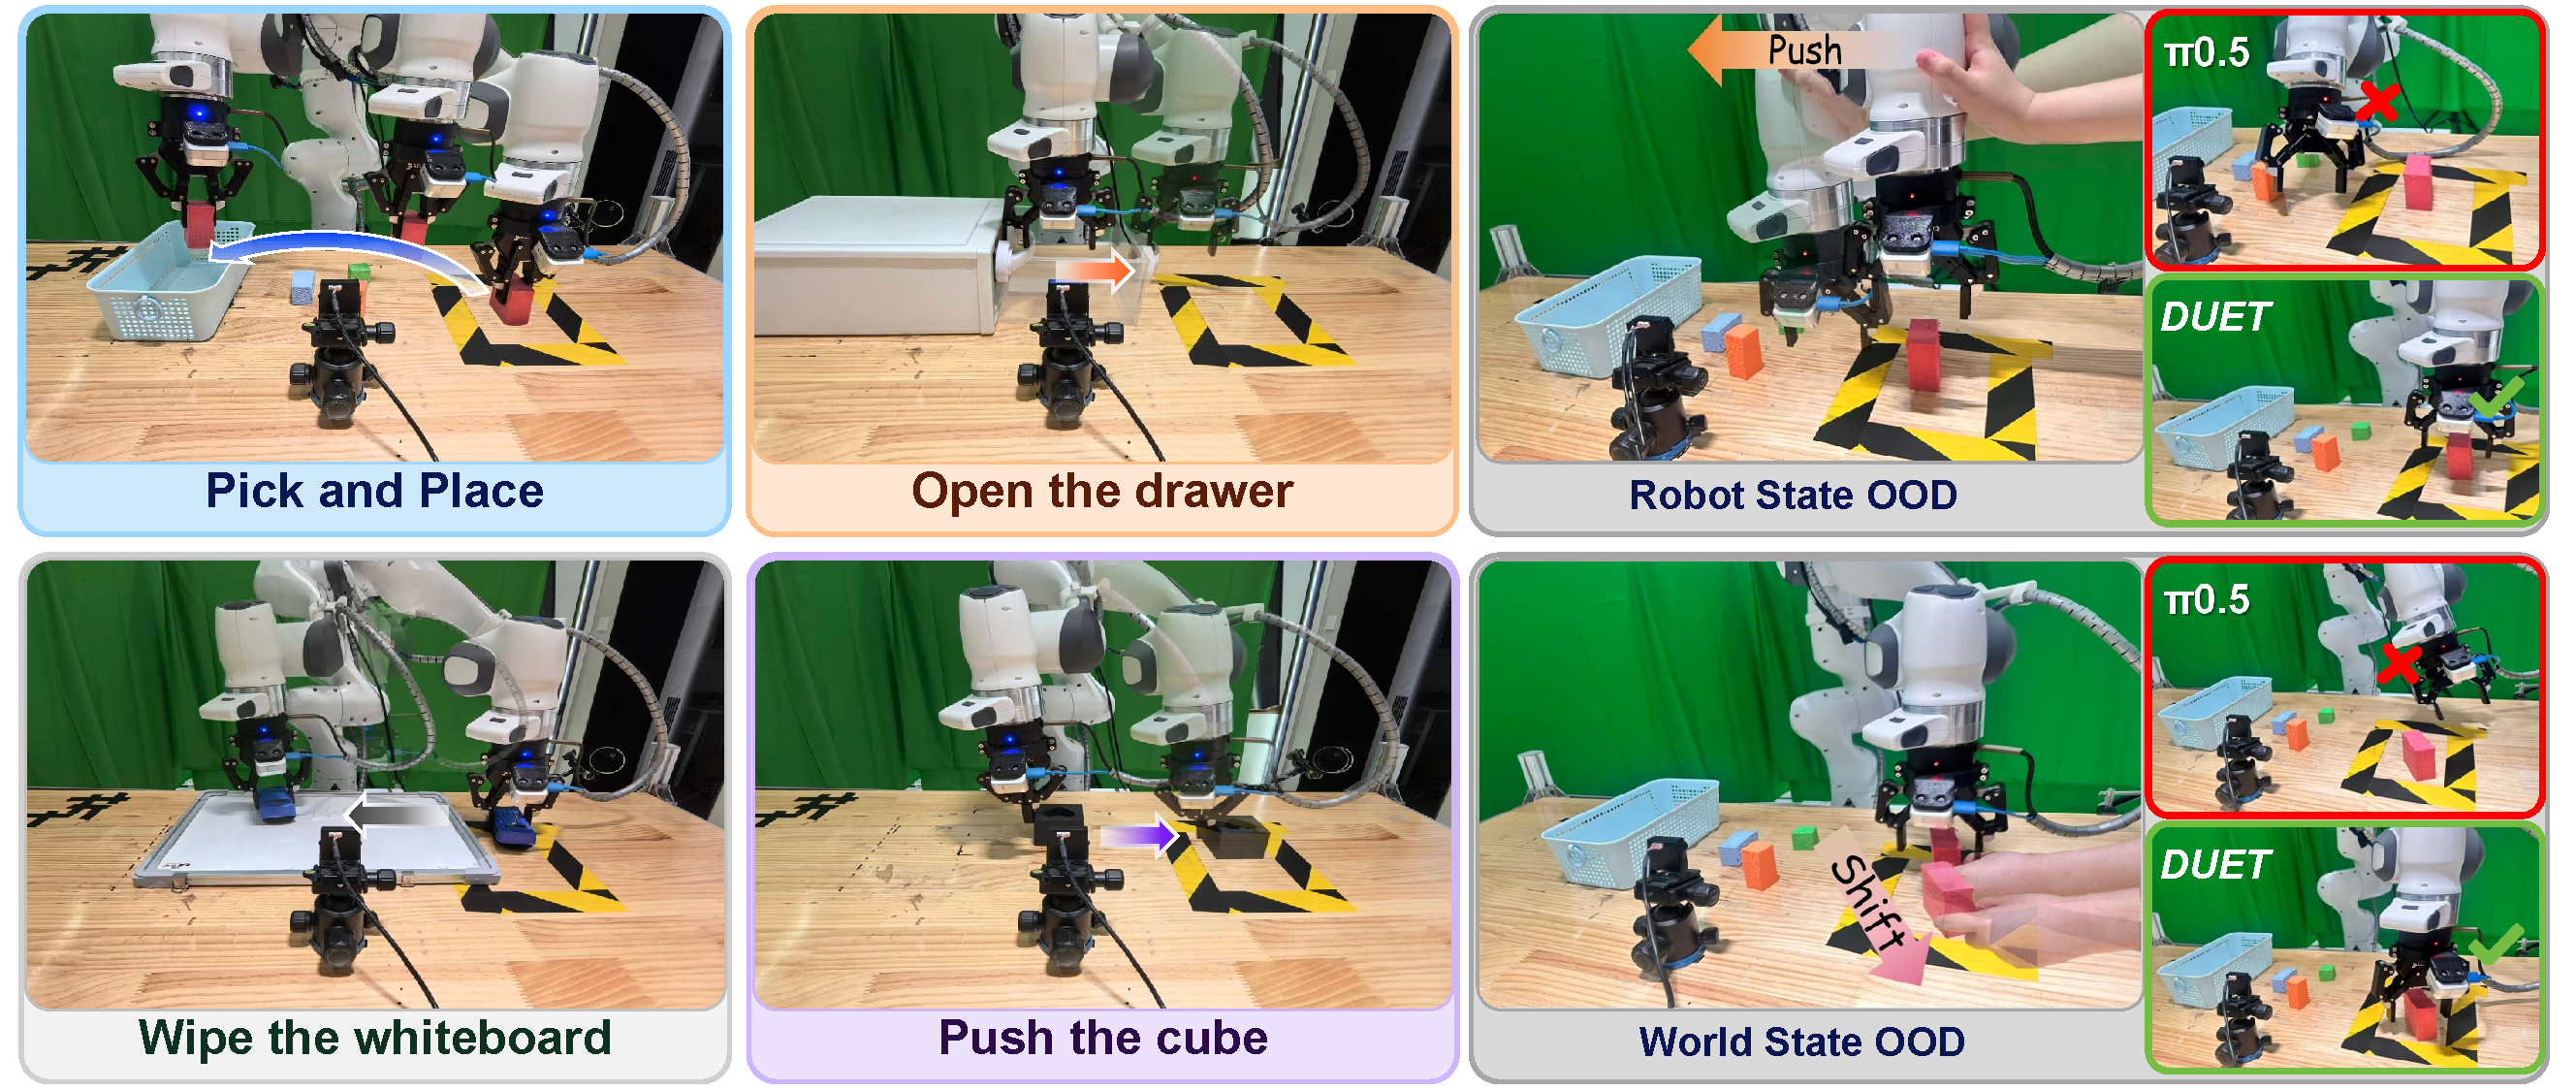
\includegraphics[width=0.96\textwidth]{figures/real-robot-exp.pdf}
\caption{Franka evaluation. Left: pick-and-place, drawer opening, wiping, and pushing. Right: pushing recovery under EEF (top) and object (bottom) shifts.}
\label{fig:real_tasks}
\end{figure*}

\subsection{\textbf{(Q3)} Endogenous Failure-Risk Scoring}
\label{sec:detection}
Table~\ref{tab:detection} evaluates $D_t$ against detectors trained without failure examples under matched rollouts \cite{faildetect,sentinel}. Matched timestep scores are split by $(\mathrm{task},\mathrm{initial\ state})$ key. For detector $m$, $\gamma_m$ is selected on the calibration split at $95\%$ TPR and frozen on the test split; labels set only this reporting point and do not train the detector. This evaluation threshold differs from controller threshold $\tau$. TPR, TNR, and AUROC use held-out timestep scores; Loc.@16 is the fraction of perturbed episodes first alarming within $16$ steps after injection. Unlike the baselines, $D_t$ also supplies correction $c_t$ and is not a calibrated failure probability.

\begin{table}[t]
\caption{Matched-protocol failure-risk scoring. Higher is better; column bests in bold.}
\label{tab:detection}
\centering
\resizebox{\columnwidth}{!}{%
\begin{tabular}{@{}lcccc@{}}
\toprule
Method & TPR $\uparrow$ & TNR $\uparrow$ & AUROC $\uparrow$ & Loc.@16 $\uparrow$ \\
\midrule
logpZO \cite{faildetect} & 0.889 & 0.243 & 0.817 & \textbf{0.569} \\
RND \cite{rnd,faildetect} & 0.842 & \textbf{0.361} & 0.549 & 0.330 \\
PCA-kmeans \cite{faildetect} & 0.884 & 0.283 & 0.625 & 0.503 \\
STAC \cite{sentinel} & 0.839 & 0.311 & 0.494 & 0.260 \\
\rowcolor{gray!20}
DUET ($D_t$) & \textbf{0.900} & 0.265 & \textbf{0.845} & 0.523 \\
\bottomrule
\end{tabular}}
\end{table}

DUET leads AUROC and TPR, whereas RND leads TNR and logpZO localization; ranking quality therefore does not guarantee fewer false alarms or earlier detection. DUET nevertheless uses a continuous correction rather than a binary stop: over $2{,}000$ clean episodes, $\alpha_t$ averages $0.139$, its $95$th percentile is $0.339$, and only $1.7\%$ of steps exceed $0.5$. Thus, $D_t$ is a competitive ranking and control signal for these deviations, not a calibrated failure probability.

\subsection{Ablations}
\label{sec:ablations}
Table~\ref{tab:main_results} shows that merely adding an absolute prediction is insufficient: absolute-only and fixed fusion severely reduce clean success, and fixed fusion underperforms DUET-Rel under action perturbation. Adaptive fusion instead reaches $84.4\%$, supporting conditional waypoint use. The four-suite displacement row uses medium severity; Table~\ref{tab:ood_detailed} pools both severities.

\begin{table}[t]
\caption{Fusion ablations (success, \%). Four-suite $N{=}2000/2000/4000$; matched Object $N{=}500$.}
\label{tab:main_results}
\centering
\resizebox{\columnwidth}{!}{%
\begin{tabular}{llccc}
\toprule
Controller & Gate & Clean & Robot displ. & Action exec. \\
\midrule
\multicolumn{5}{@{}l}{\textit{Four-suite average}} \\
DUET-Rel & $\alpha_t{=}0$ & 93.8 & 40.0 & 27.9 \\
\rowcolor{gray!20}
DUET & adaptive $\alpha_t$ & \textbf{96.9} & \textbf{61.7} & \textbf{64.6} \\
\midrule
\multicolumn{5}{@{}l}{\textit{Object suite, matched protocol}} \\
DUET-Rel & $\alpha_t{=}0$ & 99.2 & 36.2 & 48.8 \\
Absolute-only & $\alpha_t{=}1$ & 5.2 & 1.1 & 0.8 \\
Fixed fusion & $\alpha_t{=}0.5$ & 46.2 & 39.4 & 41.0 \\
\rowcolor{gray!20}
DUET & adaptive $\alpha_t$ & 99.2 & \textbf{76.0} & \textbf{84.4} \\
\bottomrule
\end{tabular}}
\end{table}

Table~\ref{tab:ablations} separates CFG from training replacements. Removing adaptive CFG or branch-specific augmentation reduces every reported outcome. RVQ-to-MLP replacement yields zero LIBERO-10 success in this configuration, not a general rejection of continuous heads; comparisons remain within each suite-specific block.


\begin{table}[t]
\caption{Component and gate-score ablations (success, \%).}
\label{tab:ablations}
\centering
\resizebox{\columnwidth}{!}{%
\begin{tabular}{lccc}
\toprule
Variant & Clean & Robot displ. & Action exec. \\
\midrule
\multicolumn{4}{@{}l}{\textit{CFG schedule, Object suite}} \\
No adaptive CFG & 88.2 & 52.6 & 57.2 \\
\rowcolor{gray!20}
Full DUET & 99.2 & 76.0 & 84.4 \\
\midrule
\multicolumn{4}{@{}l}{\textit{Training replacements, LIBERO-10}} \\
RVQ $\rightarrow$ MLP & 0.0 & 0.0 & 0.0 \\
Symmetric augmentation & 86.8 & 58.6 & 60.9 \\
\rowcolor{gray!20}
Full DUET & 91.8 & 60.8 & 63.8 \\
\midrule
\multicolumn{4}{@{}l}{\textit{Gate-score decomposition, Object (medium)}} \\
Relative only ($\alpha_t{=}0$) & 99.2 & 36.2 & 48.8 \\
$S_t$ only & 99.0 & 52.4 & 56.0 \\
$\lVert c_t\rVert_2$ only & 98.8 & 61.6 & 67.2 \\
$D_t$ only & 99.0 & 70.8 & 80.6 \\
\rowcolor{gray!20}
$D_t+\lambda S_t$ (full) & \textbf{99.2} & \textbf{76.0} & \textbf{84.4} \\
\bottomrule
\end{tabular}}
\end{table}


\paragraph{Recovery-score decomposition}
Using a shared checkpoint and matched Object rollouts, thresholds are calibrated on disjoint clean rollouts to match nominal activation. $D_t$ is the strongest individual cue; correction magnitude also grows during legitimate motion, while $S_t$ requires a bound crossing. Their combination improves on $D_t$ by $5.2$ pp under displacement and $3.8$ pp under action perturbation with unchanged clean success.

\subsection{Real-Robot Evaluation}
\label{sec:real_robot}
We test whether the DUET design applies to a separately trained $\pi_0$ (OpenPi) controller \cite{pi0}, rather than transferring simulation weights directly. A 7-DoF Franka Panda uses wrist and third-person cameras at $20$\,Hz. Each task is fine-tuned for $5$k steps from $\pi_0$-base on $50$ VR demonstrations. The four tasks are pick-and-place, pushing, drawer opening, and wiping (Fig.~\ref{fig:real_tasks}, left).

Each task is evaluated under nominal execution and two OOD families ($N{=}20$ trials per cell): a random-direction EEF shift (robot state) and an object displacement (world state), with task-specific intervention phases and magnitudes. Random directions are paired across $\pi_0$ and $\pi_0$+DUET.

% Keep the final table-to-text gap compact without changing type or margins.
\setlength{\textfloatsep}{1.2\baselineskip plus 2pt minus 2pt}
\begin{table}[t]
\caption{Franka success (\%, $\pi_0$-base; $N{=}20$/cell, $80$ overall). Robot: random-direction EEF shift; world: object shift. $\Delta$: +DUET minus $\pi_0$.}
\label{tab:real_robot}
\centering
\footnotesize
\setlength{\tabcolsep}{2.6pt}
\resizebox{\columnwidth}{!}{%
\begin{tabular}{@{}l cc ccc ccc@{}}
\toprule
& \multicolumn{2}{c}{Nominal} & \multicolumn{3}{c}{Robot-state (EEF shift)} & \multicolumn{3}{c}{World-state (Obj.\ shift)} \\
\cmidrule(lr){2-3}\cmidrule(lr){4-6}\cmidrule(l){7-9}
Task & $\pi_0$ & +DUET & $\pi_0$ & +DUET & $\Delta$ & $\pi_0$ & +DUET & $\Delta$ \\
\midrule
Pick-and-place    & 95.0 & 95.0 & 15.0 & 85.0 & $+70.0$ &  5.0 & 50.0 & $+45.0$ \\
Block pushing     & 95.0 & 90.0 & 10.0 & 75.0 & $+65.0$ &  0.0 & 60.0 & $+60.0$ \\
Drawer opening    & 95.0 & 95.0 & 10.0 & 80.0 & $+70.0$ & 20.0 & 70.0 & $+50.0$ \\
Whiteboard wiping & 75.0 & 80.0 &  5.0 & 70.0 & $+65.0$ &  0.0 & 55.0 & $+55.0$ \\
\midrule
\rowcolor{gray!20}
\textbf{Overall}  & 90.0 & 90.0 & 10.0 & \textbf{77.5} & $\mathbf{+67.5}$ & 6.3 & \textbf{58.8} & $\mathbf{+52.5}$ \\
\bottomrule
\end{tabular}}
\end{table}

DUET preserves $90.0\%$ aggregate nominal success (Table~\ref{tab:real_robot}). Robot-state OOD rises from $10.0\%$ to $77.5\%$ (Wilson $95\%$ CIs: $5.2$--$18.5\%$, $67.2$--$85.3\%$), and world-state OOD from $6.3\%$ to $58.8\%$ ($2.7$--$13.8\%$, $47.8$--$68.9\%$). Because interventions are task-specific and each cell has $20$ trials, these results support the evaluated tasks and backbone rather than broad cross-robot generalization. No additional detector or recovery data are used.

\section{DISCUSSION}

Shared-checkpoint comparisons isolate adaptive fusion, while ablations show that neither waypoints nor geometric re-entry alone ensure completion. DUET works best when the visual target remains valid; changed object relations are harder. It is a retry controller for recoverable execution deviations, not a semantic replanner or universal detector.

\section{LIMITATIONS}

DUET requires aligned absolute-state labels and controller-scale calibration. Coordinatewise bounds ignore multimodal structure, while the state-excluded absolute head can miss hidden information. Shared visual corruption and changed object relations weaken $D_t$; invalid images require the guard. Fixed-phase interventions test one recovery horizon, and thresholds require deployment recalibration. Simulation uses one seed; hardware covers one robot with $20$ trials per cell. Irreversible failures and new-strategy cases remain out of scope.

\section{CONCLUSION}

DUET couples failure-risk scoring and correction by comparing relative commands with success-trained absolute waypoints. Its gate preserves nominal control while improving recovery from controlled execution deviations, without an external detector or recovery demonstrations. Separately trained StarVLA and $\pi_0$ controllers support applicability across two backbones; broader generalization remains future work.

% Keep all floats ahead of the references without forcing an extra page.
\FloatBarrier
\balance
\bibliographystyle{IEEEtran}
\bibliography{references}

\end{document}
